\setcounter{chapter}{20}
\chapter{Synthèse Organique (partie 1)}
\section{Optimisation d'une étape de synthèse}
\subsection{Rappels}

On a décrit les réactions chimiques suivant deux aspects:
\begin{itemize}
	\item cinétique: influence des facteurs cinétiques (\trou{température}, \trou{catalyseur})
	\item rendement: c'est le rapport entre la quantité de produit expérimentalement produit et la quantité de produit que l'on produirait si la \trou{réaction était totale}.\
\end{itemize}
\blocrouge{A SAVOIR}{
Il y a deux techniques permettant d'augmenter le rendement d'une réaction:
\begin{enumerate}
	\item Introduire un \trou{réactif en excès}.
	\item Eliminer un \trou{produit} au fur et à mesure de se formation dans le milieu réactionnel.
\end{enumerate}
}
\subsection{Application}

On considère une réaction d'estérification (synthèse d'un ester). 
\begin{center}
	alcool + acide $\leftrightharpoons$ ester + eau
\end{center}

Cette réaction est un équilibre dont la constante vaut K=4,00. Les réactifs et produits sont en phase liquide. On assimilera leurs activités à leurs quantités de matière.

\etiquette{Protocole expérimental}
On introduit dans un ballon:

\begin{minipage}{.60\textwidth}

\begin{itemize}
	\item 8,5 mL d'acide éthanoïque ;
	\item 21,4 mL de 3-méthylbutan-1-ol ;
	\item 10 mL de cyclohexane ;
\end{itemize}
On réalise le montage de \trou{Dean-Stark} avec  la colonne graduée remplie de cyclohexane. On règle le chauffage au maximum. On arrête le chauffage lorsque 2,2 mL de liquide ont été recueillis en dessous du cyclohexane dans la colonne du Dean-Stark. Le cyclohexane et l'eau ne sont  pas miscibles.

\end{minipage}
\hfill
\begin{minipage}{.35\textwidth}
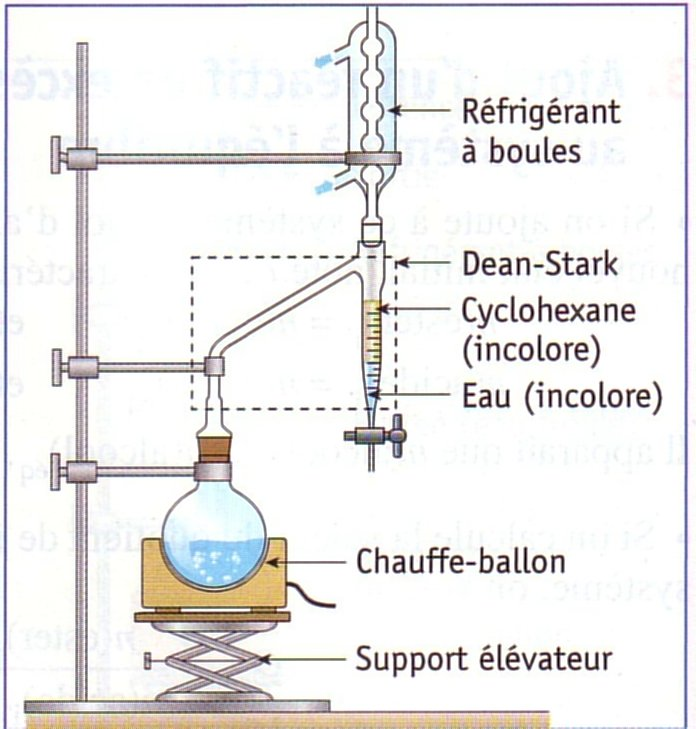
\includegraphics{figures/dean_stark}
\end{minipage}





\begin{tabular}{|l|c|c|c|c|c|}
\hline
Données &Acide éthanoïque & 3-méthylbutan-1-ol &Ester&cyclohexane & Eau\\
  \hline
  Masse molaire en g/mol & 60&88 &130 &78 &18\\
Densité  &1.05 &0.81 &0.87 & 0.88 & 1.00 \\
$\theta_{ebullition}$ & 118 & 138 & 142 & 81 & 100 \\
\hline
\end{tabular}

\etiquette{Questions}
\begin{enumerate}
	\item Déterminer les quantités de matières des deux réactifs à l'état initial. (Solution: $n_{acide}=\SI{149}{\milli \mol}$ ;  $n_{alcool}=\SI{197}{\milli \mol}$)
	\item Calculer la quantité maximale $n_{max}$ d'eau formée. (Solution: $n_{max}=\SI{149}{\milli \mol}$ )
	\item En déduire la valeur du rendement de cette réaction avec extraction de l'eau.  ($\eta = .82 = 82\%$)
	\item Déterminer l'avancement final $x_f$ de la transformation si elle avait lieu  sans extraction. (Solution: $x_f=\SI{112}{\milli\mol}$)
	\item Calculer le rendement sans extraction. (Solution: $75\%$)
	\item Pourquoi parle-t-on de déplacement d'équilibre lorsque l'on retire l'eau à l'aide de la colonne de Dean-Stark ?
\end{enumerate}

\etiquette{Vidéo du montage}
\url{https://youtu.be/_zbHeEtRTZw?si=klHvdfqU5bZK3eoG}
%\newpage

\section{Stratégie de synthèse multi-étapes}
\subsection{Grands types de réactions}

Parmi les 5 types de réaction, on connaît déjà: 
\begin{itemize}
	\item \trou{Oxydoréduction}: échange d'électrons
	\item \trou{Acide-base}: échange de protons ($H^+$)
\end{itemize}
En voici 3 autres:

\etiquette{Addition} Une molécule qui possède une \trou{double liaison} et s'associe avec une autre molécule pour réagir.

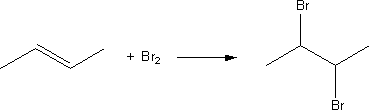
\includegraphics[scale=.80]{figures/addition}

\etiquette{Elimination} Une molécule se  scinde en deux dont l'une possède un \trou{double liaison}.

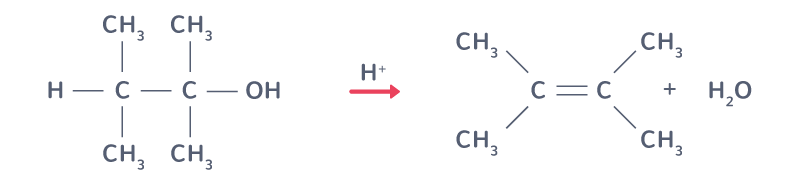
\includegraphics[scale=.40]{figures/elimination}

\etiquette{Substitution} Un atome ou un groupe d'atomes d'une molécule est \trou{remplacée} par un autre atome ou groupe d'atomes.

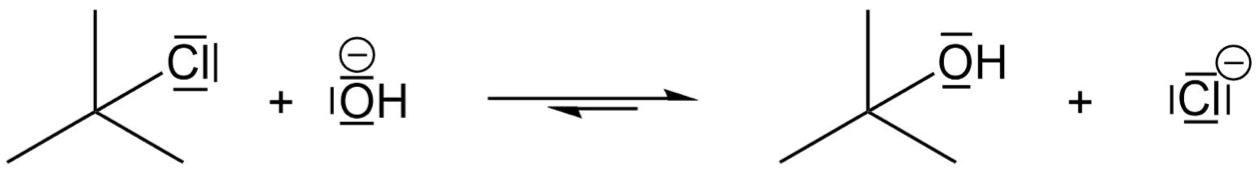
\includegraphics[scale=.450]{figures/substitution}

\subsection{Protection - Déprotection}

On considère une molécule avec plusieurs groupes fonctionnels susceptibles de réagir face à un réactif. On peut bloquer la réactivité d'un de ces groupes en réalisant la séquence suivante:

\begin{enumerate}
	\item \trou{Protection} du groupement pour lequel on ne souhaite pas de transformation chimique ;
	\item Action du réactif sur la molécule dont un groupement est protégée ; 
	\item \trou{Déprotection}: réaction permettant de régénérée le groupe fonctionnel initialement modifié par la réaction de protection.
\end{enumerate}

\etiquette{Exemple} Exercice 28 p 207

\begin{minipage}{.45\textwidth}
  On étudie la synthèse multi-étapes de B' à partir du réactif A. Pour cela, on doit modifier le groupe ester en groupe hydroxyle sans faire réagir le groupe cétone. 
\begin{enumerate}
	\item Quels sont  les groupes présents dans la molécule A. Comment se nomme ce type de composé ?
	\item Les réactifs $LiAlH_4$ et $NaBH_4$ ont ils les mêmes effets sur la molécule A ?
	\item Comment  se nomme l'étape 1 ? Quel est son intérêt ?
	\item Comment se nomme l'étape 3  ?
	\item Quel
\end{enumerate}  
  \end{minipage}
\hfill
\begin{minipage}{.55\textwidth}
\includegraphics[width=\textwidth]{figures/Exoprotection.pdf}
\end{minipage}


\subsection{Chimie Verte}

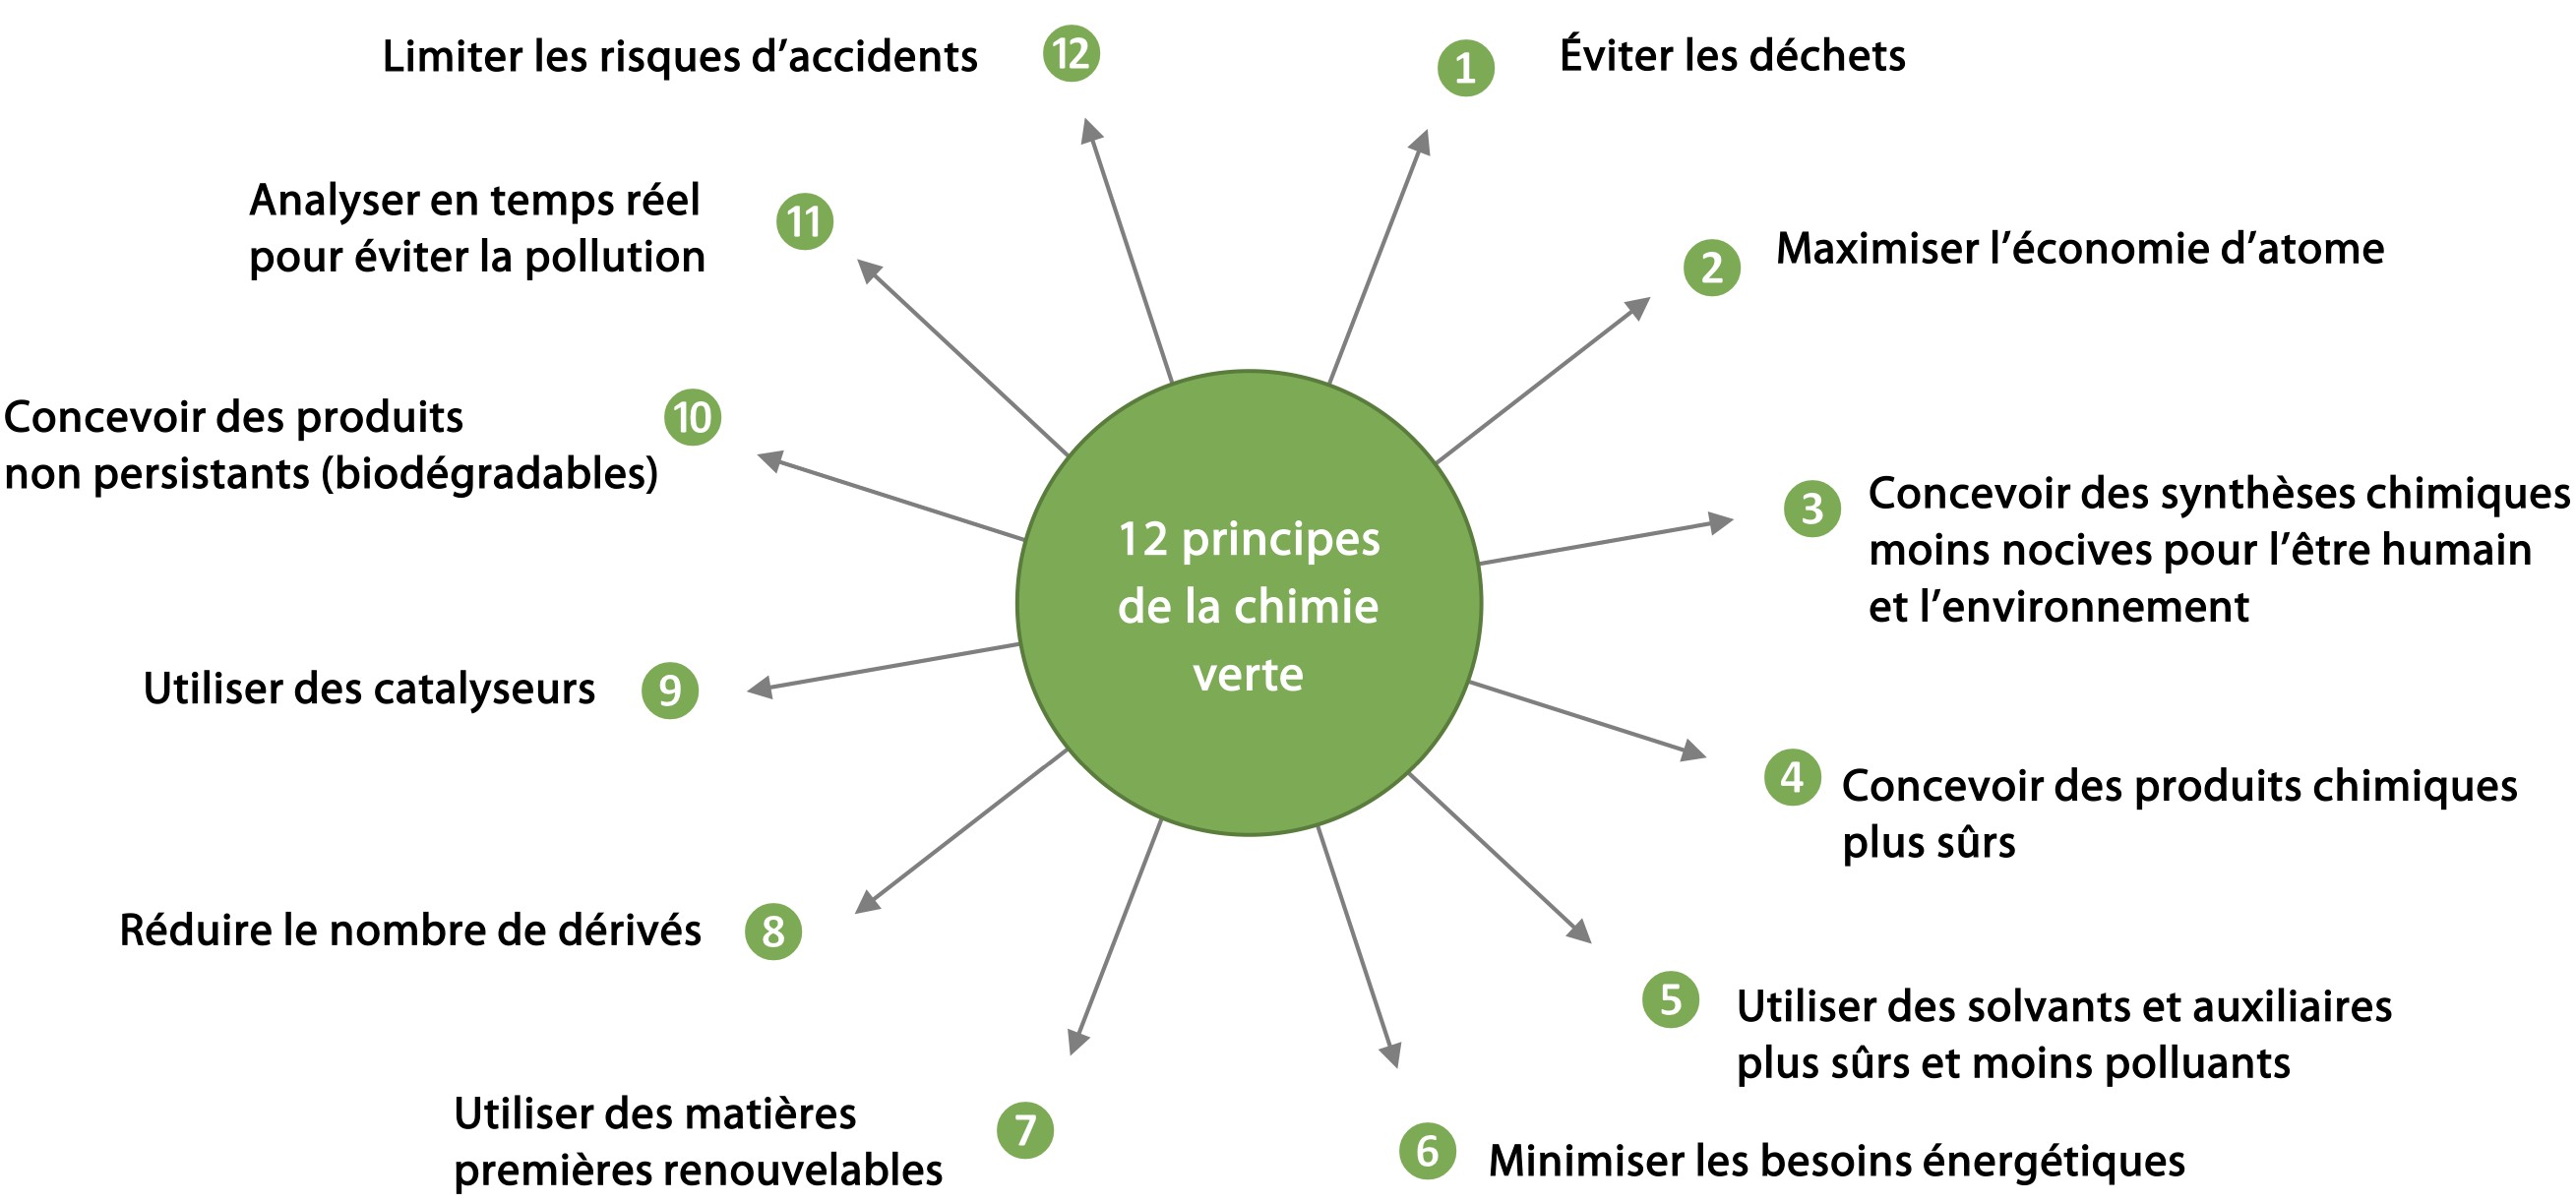
\includegraphics[width=.95\textwidth]{figures/chimie_verte}

\begin{travail}
\begin{itemize}
	\item Formules semi-développées, topologiques: 4, 5 p 202
	\item Rendement: 32 p 210 -  Protection: 33 p 211 - Dean Stark: Préparation ECE p 211
		\item Type BAC: \url{https://www.labolycee.org/synthese-dun-arome-dorange} BAC 2022
	\item Type BAC: \url{https://www.labolycee.org/synthese-dun-arome} BAC 2021

\end{itemize}
\end{travail}
